\documentclass{../papanleitung}

\def\versuchnr{251}
\def\versuchshorttitle{Statistik}
\def\versuchtitle{Statistik des radioaktiven Zerfalls}

\begin{document}

\begin{figure}[h]
\begin{minipage}[c]{12cm}
\centering\epsfig{file=251_aufbau.eps,width=\textwidth}
\caption{\fontsize{10}{12}\it Versuchsaufbau.}
\end{minipage}
\end{figure}


\section{Messaufbau}
\begin{itemize}
 \item  Geiger-M\"{u}ller Z\"{a}hlrohr mit Betriebsger\"{a}t
 \item  externer Impulsz\"{a}hler
 \item PC mit Drucker
 \item Pr\"{a}paratehalterung mit Bleiabschirmung
 \item Radioaktives Pr\"{a}parat ($^{60}$Co oder $^{137}$Cs)
\end{itemize}

\section{Literatur}

\begin{itemize}
 \item W.~Walcher,  \it{Praktikum der Physik}\rm, B.G.Teubner
 Stuttgart.
\item J. Stiewe, \it Wir wollen richtige Fehler\rm, der
Praktikumsanleitung beigef\"{u}gt.
 \item  Homepage des Praktikums
(http://www.physikpraktika.uni-hd.de).
\end{itemize}





\section{Vorbereitung}
Bereiten Sie sich  auf die Beantwortung von Fragen zu folgenden
Themen vor: Grundlagen der Wahrscheinlichkeitsrechnung und Statistik, Radioaktiver Zerfall,
Geiger-M\"{u}ller-Z\"{a}hlrohr.\\
\\Verst\"{a}ndnisfragen:
\begin{enumerate}
\item  Was ist Radioaktivit\"{a}t?\item Wie lautet das
Zerfallsgesetz? \item Was ist ein Isotop? \item In welcher
Beziehung stehen die Binomial-, Poisson- und Gau{\ss}-Verteilung?
\item Wodurch wird die mit einem Z\"{a}hlrohr gemessene
Z\"{a}hlrate bestimmt? Warum muss die Messung im Plateaubereich
durchgef\"{u}hrt werden?\item An einer Probe eines langlebigen
radioaktiven Materials werde als Mittel einer Reihe von 20
Messungen eine Rate von 23,5 Zerf\"{a}llen pro 10~s gemessen.
\begin{enumerate}
\item [a)] Wie gro{\ss} ist die Varianz dieser Verteilung? \item [b)]
Wie gro{\ss} ist der Fehler des Mittelwertes?
\end{enumerate}
\item Die Gr\"{o}{\ss}e von 4402 Studenten sei normalverteilt mit einem
Mittelwert von 185~cm und einer Standardabweichung von 3~cm.
\begin{enumerate}
\item [a)] Wie viele dieser Studenten haben eine Gr\"{o}{\ss}e zwischen
179~cm und 188~cm? \item [b)] Wie viele sind gr\"{o}{\ss}er als 191~cm?
\end{enumerate}
\end{enumerate}
\section{Aufgaben}
\begin{enumerate}
\item Messen Sie ausgehend von der Einsatzspannung bis 100~V
dar\"{u}ber die Z\"{a}hlrohrcharakteristik. \item Untersuchen Sie den
Anstieg der Z\"{a}hlrate im Plateau des Z\"{a}hlrohrs unter
Ber\"{u}cksichtigung der statistischen Schwankungen.

\item Anhand einer langen Messreihe sind die Schwankungen der
Z\"{a}hlrate experimentell zu untersuchen und damit die statistische
Natur des radioaktiven Zerfalls zu best\"{a}tigen. Die Messdaten sollen
mit einer mit einer Poisson- und
Gauss- Verteilung verglichen werden.
 \item Wiederholen
Sie die zuvor durchgef\"{u}hrte Messung bei einer sehr niedrigen
Z\"{a}hlrate und vergleichen Sie die Messdaten mit einer Poisson- und
Gauss- Verteilung.
\end{enumerate}

\section{Motivation}
\bf Radioaktive Atome tragen in sich eine geheimnisvolle innere
     Statistik-Uhr\newline\newline
\it\glqq
     Ein Atom ist zwar bekanntlich nicht unteilbar, doch alles in allem
     sehr stabil. Die allermeisten Atome in unserer Welt existieren bereits
     seit Milliarden von Jahren. Sie wurden irgendwann im Inneren eines
     Sterns erbr\"{u}tet. Doch es gibt auch instabile Atome, die nicht f\"{u}r die
     Ewigkeit gemacht sind. Ohne jeden \"{a}u{\ss}eren Einfluss k\"{o}nnen sie ganz
     spontan zerfallen. Solche Atome nennt man radioaktiv. Beim Zerfall
     senden sie Strahlung aus - Helium\-atomkerne (Alpha-Strahlung),
     Elektronen (Beta-Strahlung) oder energiereiche elektromagnetische
     Wellen (Gamma-Strahlung). Betrachtet man ein einzelnes radioaktives
     Atom, so kann niemand vorhersagen, auch der beste Physiker nicht, wann
     dieses Atom zerfallen wird. Das kann in der n\"{a}chsten Sekunde
     geschehen, in einem Monat oder in tausend Jahren. Die \glqq innere
     Uhr\grqq~
     eines radioaktiven Atoms kennen wir nicht. Und doch gehorcht der
     Zerfall radioaktiver Atome pr\"{a}zisen Gesetzen der Statistik. So l\"{a}sst
     sich genau vorhersagen, wie sich Kollektive aus vielen Atomen
     verhalten werden, auch wenn das Schicksal jedes Einzelatoms nicht
     vorhersehbar ist. Nach einer ganz bestimmten Zeit, der so genannten
     Halbwertszeit, ist stets die H\"{a}lfte aller zun\"{a}chst vorhandenen Atome
     zerfallen. Die Halbwertszeit ist dabei ein f\"{u}r jede Sorte radioaktiver
     Atome charakteristischer Wert. Das Isotop Jod-131 besitzt zum Beispiel
     immer eine Halbwertszeit von 8,02 Tagen. Manche Atome sind so
     instabil, dass ihre Halbwertszeit nur Bruchteile von Sekunden betr\"{a}gt.
     Nach nur 1,05 Millionstel Sekunden sind beispielsweise 50 Prozent der
     Thorium-219-Atome zerfallen. Auch das andere Extrem gibt es. Uran-235,
     das zum Bau von Atombomben verwendet wird, hat eine Halbwertszeit von
     mehr als 700 Millionen Jahren.\grqq\rm\footnote{Norbert
     Lossau, Artikel vom 18. August
     2004 in der Zeitung \glqq Die Welt\grqq}\newline



\section{Grundlagen}


\subsection{Wahrscheinlichkeitsverteilungen}
Misst man mit einem Z\"{a}hlrohr die von einem radioaktiven Pr\"{a}parat
emittierten Teilchen unter unver\"{a}nderten Versuchsbedingungen, so
wird man in der Regel bei jeder Messung eine etwas andere
Teilchenzahl erhalten. Der Grund hierf\"{u}r ist, dass jeweils w\"{a}hrend
der Messzeit nur ein kleiner Bruchteil der radioaktiven Atome
zerf\"{a}llt, und dass die einzelnen Zerfallsprozesse v\"{o}llig \bf
unabh\"{a}ngig\rm~ voneinander stattfinden. Die genaue Anzahl der
innerhalb der Messzeit zerfallenden Atome bleibt daher dem Zufall
\"{u}berlassen.


\begin{figure}
\begin{minipage}[c]{12cm}
\centering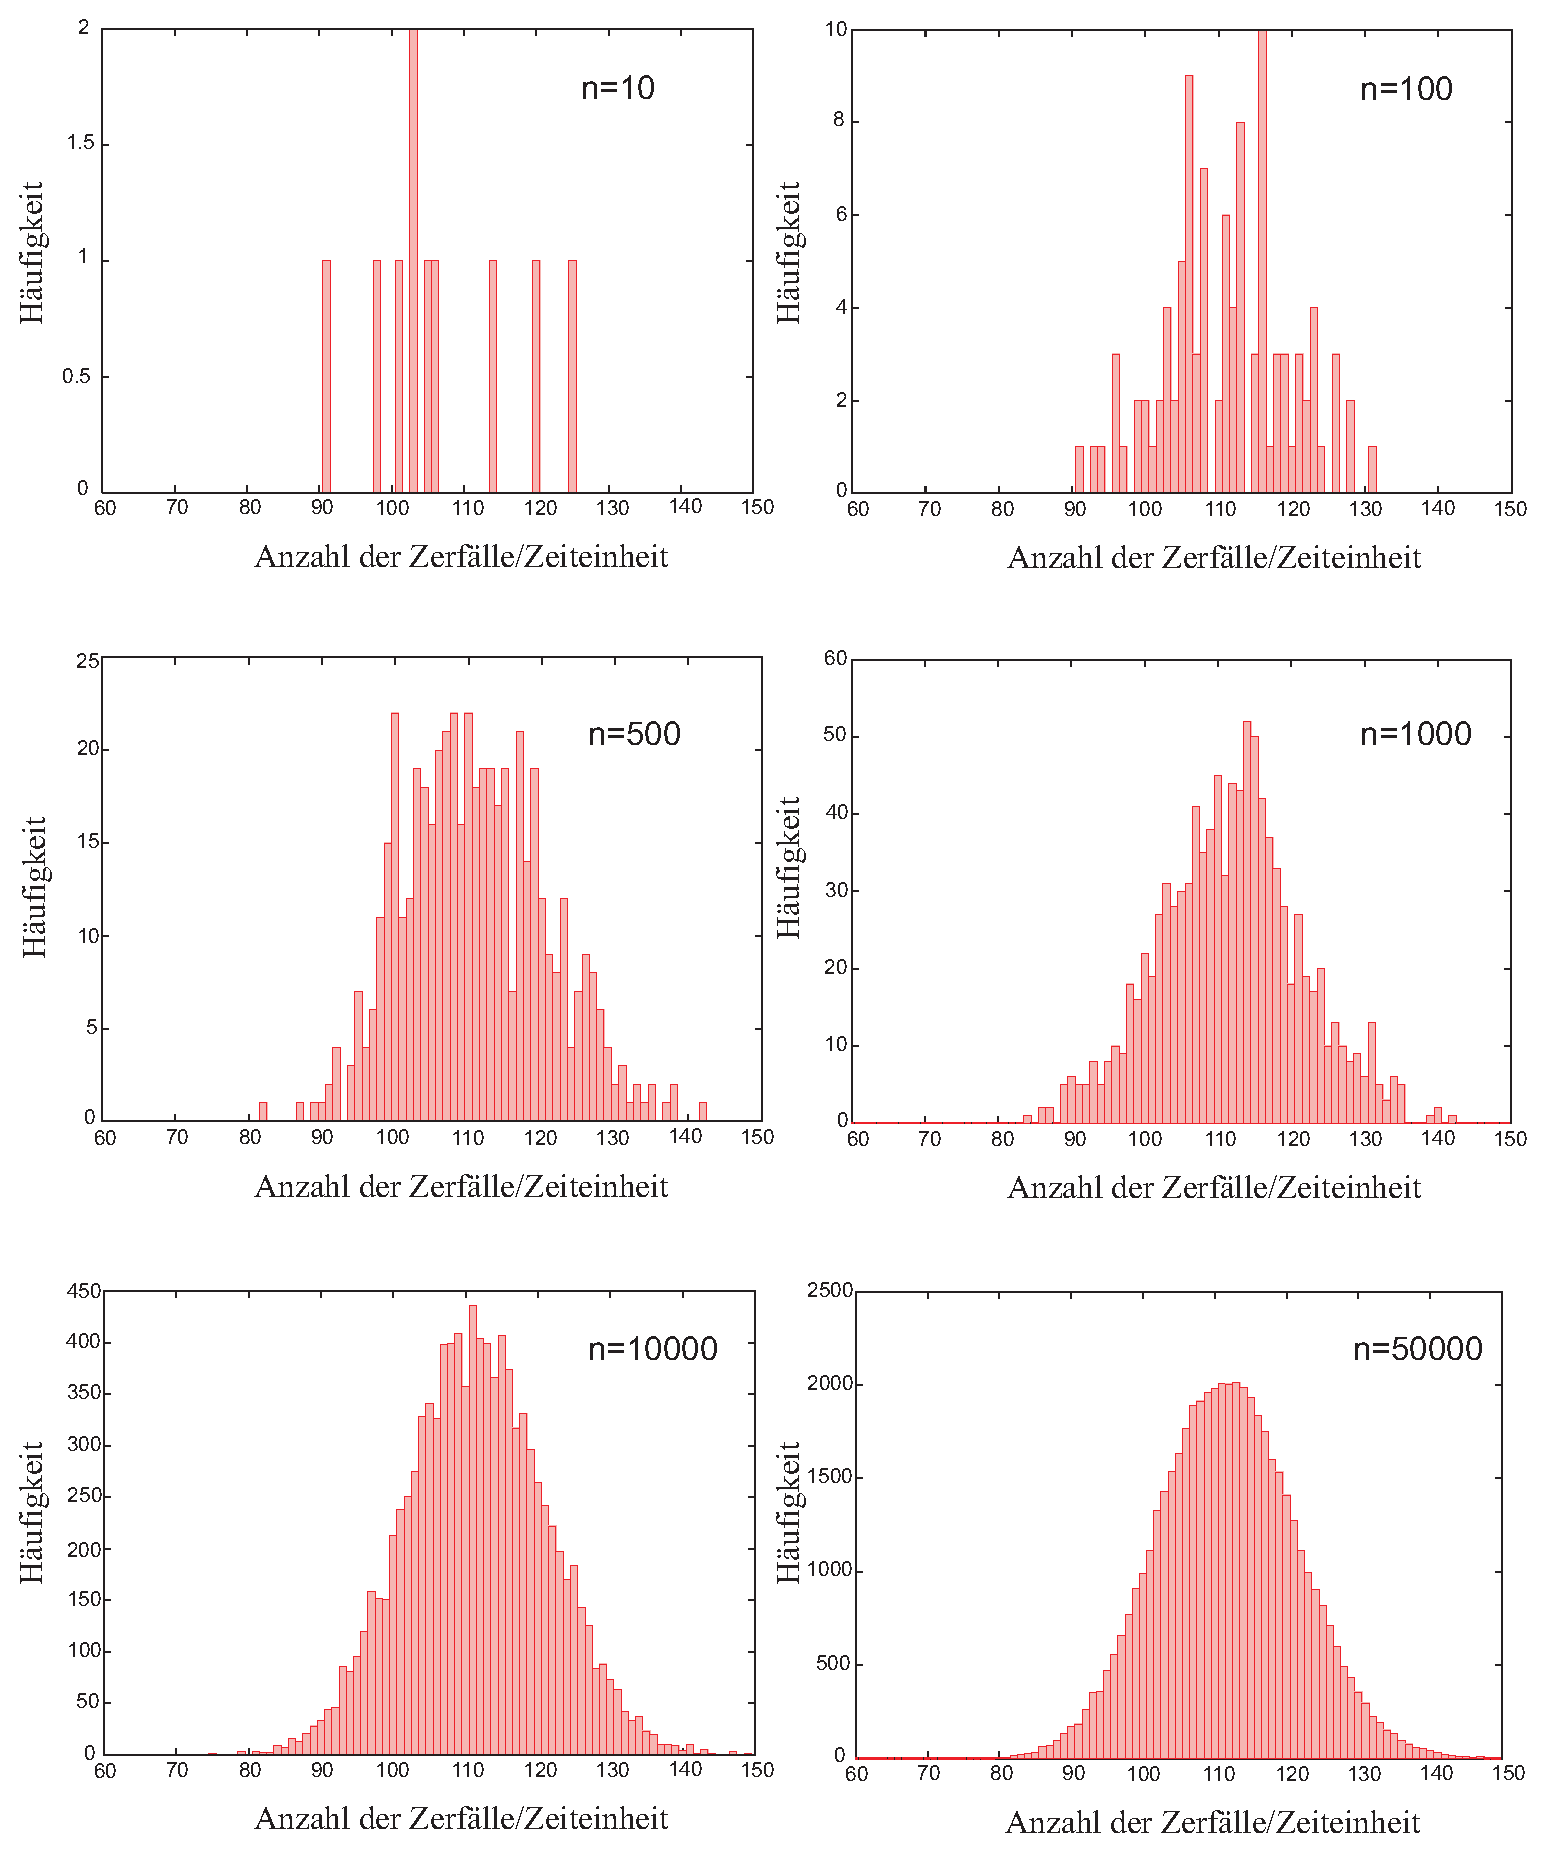
\epsfig{file=251_histo.eps,width=\textwidth}
\caption{\fontsize{10}{12}\it Tr\"{a}gt man die pro Zeiteinheit
gemessenen radioaktive Zerf\"{a}lle einer gro{\ss}en Anzahl von Atomen in
ein Histogramm ein, so erh\"{a}lt man nach vielen Messungen stets
dieselbe Verteilung. $n$ bezeichnet die Anzahl der
Messungen.\label{251_histo}}
\end{minipage}
\end{figure}

Allerdings l\"{a}sst sich mit dem Zufall hervorragend
experimentieren und rechnen. Der Zufall zeigt
Gesetzm\"{a}{\ss}igkeiten!~Zwar ist es unm\"{o}glich den
Zerfallszeitpunkt eines \bf einzelnen\rm~Atomkernes vorherzusagen
- \"{u}ber \bf eine gro{\ss}e Anzahl\rm~ von Kernen lassen sich
dagegen durchaus Vorhersagen treffen. Tr\"{a}gt man beispielsweise
die mit einem Z\"{a}hlrohr gemessene Z\"{a}hlrate in ein
Histogramm ein und wiederholt dieses viele Male, so wird man unter
bestimmten Voraussetzungen\footnote{Die Halbwertszeit des
radioaktiven Isotops muss gro{\ss} gegen\"{u}ber der
Beobachtungszeit sein.} stets dieselbe Verteilung erhalten
(Vergleiche Abbildung~\ref{251_histo}). In den folgenden
Abschnitten wollen wir untersuchen, welche statistische
Verteilungen geeignet sind
den radioaktiven Zerfall zu beschreiben.\\
\newline \it \glqq Alle Dinge umfa{\ss}t eine bestimmte Ordnung und was den ihm
angewiesenen Platz verl\"{a}{\ss}t, das tritt damit zwar in den Bereich
einer anderen Ordnung ein, aber niemals f\"{a}llt es v\"{o}llig aus aller
Ordnung heraus, denn Willk\"{u}r und Zufall sind unbekannt im Reiche
der Vorsehung!\grqq

\medskip \rm Nach: \small Boethius Anicius Manlius
Severinus: Die Tr\"{o}stungen der Philosophie\normalsize


\subsubsection{Die Binomial-Verteilung}
Die Binomial-Verteilung ergibt sich aus folgender
Fragestellung:\medskip

\textsf{Wie gro{\ss} ist die Wahrscheinlichkeit daf\"{u}r, dass ein
Ereignis \textsc{A} bei $n$ voneinander unabh\"{a}ngigen Versuchen
genau $k$-mal eintritt, wenn $p$ die Wahrscheinlichkeit f\"{u}r das
Eintreten des Ereignisses \textsc{A} bei einem Versuch ist  und
$(1-p)$ die Wahrscheinlichkeit f\"{u}r das Nichteintreten dieses
Ereignisses darstellt?} \rm\newline
\newline

Nehmen wir zun\"{a}chst an, dass das Ereignis \textsc{A} gerade
bei den ersten $k$ Versuchen  eintritt, bei den folgenden $n-k$
dagegen nicht. Da die Versuche voneinander statistisch
unabh\"{a}ngig sein sollen, m\"{u}ssen die Wahrscheinlichkeiten
f\"{u}r die einzelnen Versuche multipliziert werden. Somit ergibt
sich f\"{u}r die Wahrscheinlichkeit $W$ dieses konkreten Beispiels:
\begin{equation}
W=p^k (1-p)^{n-k}.
\end{equation}
Das Ereignis \textsc{A} muss aber nicht unbedingt bei den ersten
$k$ Versuchen auftreten. Es muss nur innerhalb von $n$ Versuchen
genau $k$-mal vorkommen. Die Reihenfolge ist dabei beliebig. Nun
gibt es aber genau $\binom{n}{k}$ M\"{o}glichkeiten, aus
$n$~Elementen $k$ herauszugreifen. Unter Beachtung aller m\"{o}glichen
Permutationen $\binom{n}{k}$ erhalten wir schlie{\ss}lich die
Binominal-Verteilung:
\begin{equation}
B(k;n,p)=\binom{n}{k}p^k (1-p)^{n-k}.
\end{equation}

Dazu folgendes Beispiel: Wie gro{\ss} ist die Wahrscheinlichkeit,
dass bei zehnmaligem W\"{u}rfeln genau dreimal die Zahl \glqq
4\grqq~f\"{a}llt?
\begin{eqnarray}
&&\text{aus}\quad p=1/6,\quad n=10 \quad\text{und}\quad k=3\quad\text{folgt:} \notag\\
&&B(3;10,1/6)=\binom{10}{3}\biggl(\frac{1}{6}\biggr)^3\biggl(1-\frac{1}{6}\biggr)^{10-3}=
15,5\%\notag
\end{eqnarray}



Die Binomial-Verteilung ist eine diskrete\footnote{d.h.
$n,k\in\mathbb{N}$}, zweiparametrische Verteilung mit den
Parametern $n$ und $p$. Als Notation verwenden wir die Bezeichnung
$B(k;n,p)$. Dabei kennzeichnet das K\"{u}rzel $B$, dass es sich um
eine Binomial-Verteilung handelt. In der Klammer wird zun\"{a}chst die
Variable angegeben, anschlie{\ss}end - getrennt durch ein Semikolon -
die Parameter.\\
\newline
Eigenschaften der Binomial-Verteilung:
\begin{alignat}{2}
&\text{Normierung:}  \quad  &  &\sum_{k=0}^n B(k;n,p)=1  \\
&\text{Mittelwert:}  \quad  &\langle k \rangle =&\sum_{k=0}^n k\,B(k;n,p) = np \\
&\text{Varianz:}    \quad &\sigma^2=&\sum_{k=0}^n
k^2\,B(k;n,p)-\langle k \rangle^2= np\,(1-p)\\
&\text{Standardabweichung:}\quad &\sigma=&\sqrt{np\,(1-p)}
\end{alignat}

Unsere bisherigen \"{U}berlegungen zur Binomial-Verteilung lassen
sich nun einfach auf den radioaktiven Zerfall \"{u}bertragen. Auch
hier handelt es sich um ein Ereignis mit zwei m\"{o}glichen Ausg\"{a}ngen:
Entweder ein radioaktiver Atomkern zerf\"{a}llt innerhalb eines
gewissen Beobachtungszeitraums oder eben nicht. Stellt $p$ die
Zerfallswahrscheinlichkeit eines Atomkerns dar, so beschreibt die
Binom\-ial-Verteilung die Wahrscheinlichkeit, dass von $n$
Atomkernen, genau $k$ innerhalb eines bestimmten Zeitraums $t$
zerfallen.

\begin{figure}
\begin{minipage}[c]{12cm}
\centering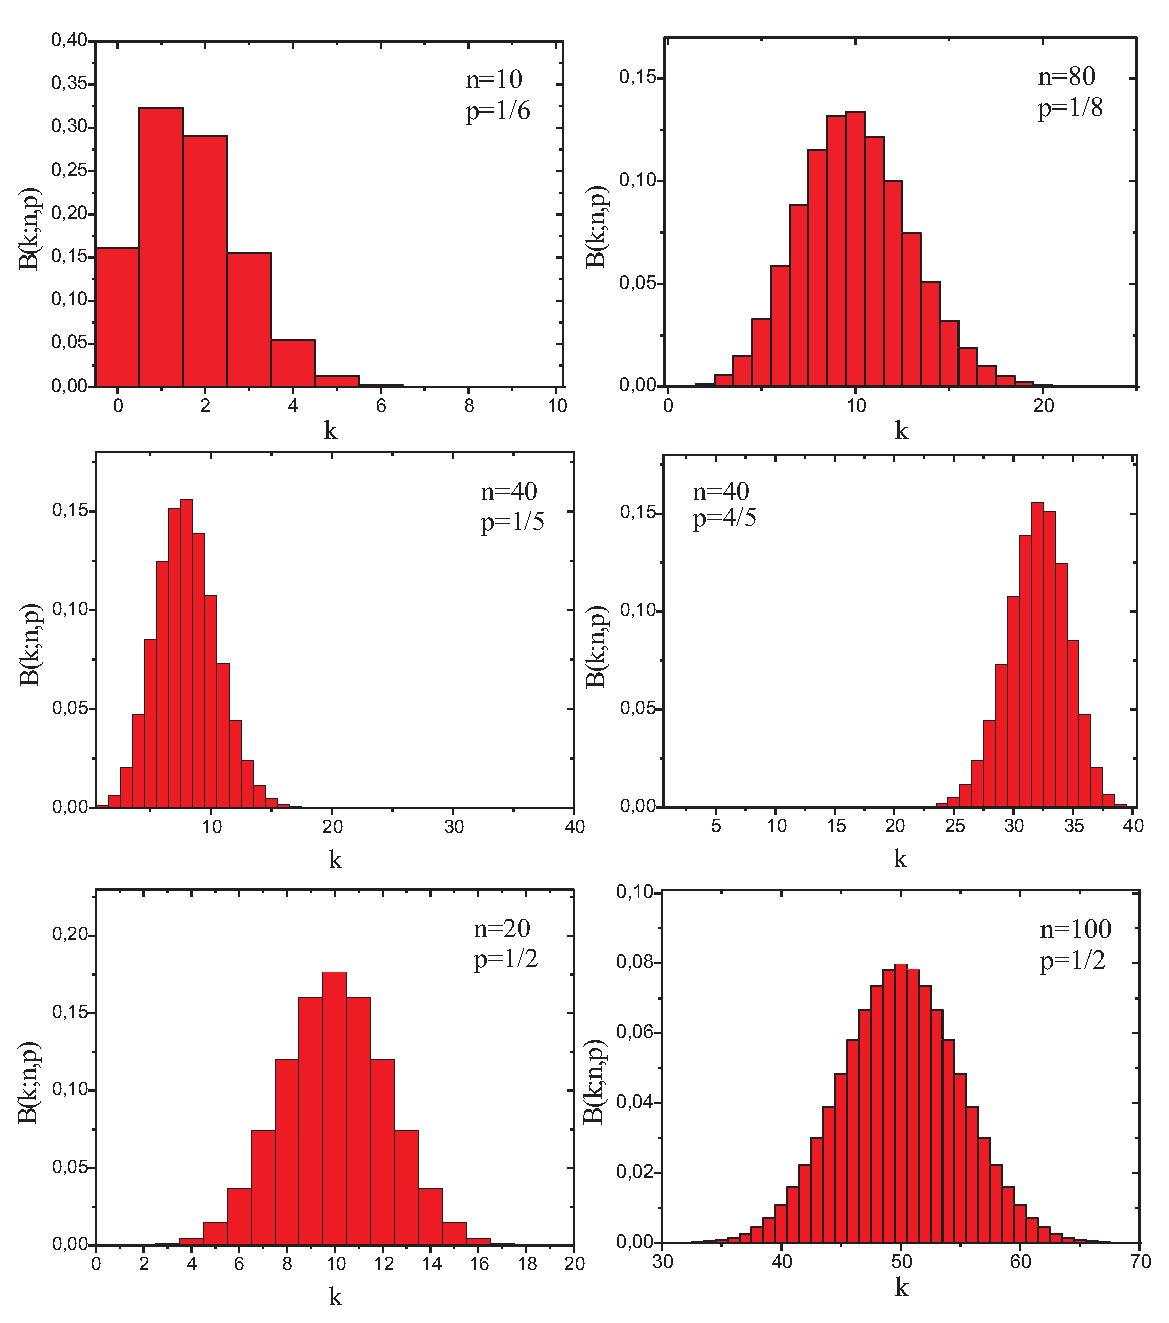
\epsfig{file=251_binom.eps,width=\textwidth}
\caption{\fontsize{10}{12}\it Binomial-Verteilung f\"{u}r
unterschiedliche Werte von $n$ und $p$.}
\end{minipage}
\end{figure}



Die Zerfallswahrscheinlichkeit $p$ h\"{a}ngt nat\"{u}rlich vom
Beobachtungszeitraum ab. Je l\"{a}nger Sie warten, desto mehr Zerf\"{a}lle
werden Sie beobachten. Es l\"{a}sst sich leicht zeigen, dass f\"{u}r $p$
gilt:
\begin{equation}\label{251_alpha}
p(t)=1-\text{e}^{-\lambda\,t},
\end{equation}
wobei die Zerfallskonstante $\lambda$ eine f\"{u}r das Isotop
charakterische Gr\"{o}{\ss}e darstellt. Sie werden diesen Sachverhalt in
dem n\"{a}chsten Praktikumsversuch, \glqq Aktivierung von Indium und
Silber mit langsamen Neutronen\grqq, noch genauer untersuchen. Ist
die Zerfallskonstante sehr klein, wie es bei den in diesem Versuch
verwendeten radioaktiven Pr\"{a}paraten der Fall ist, so kann die
Zerfallswahrscheinlichkeit $p$ f\"{u}r einen festen
Beobachtungszeitraum als konstant angenommen werden.


Obwohl die Binomial-Verteilung die Statistik des radioaktiven
Zerfalls sehr gut beschreibt, ist sie in der Praxis nur schwer
handzuhaben. Stellen sie sich vor, sie  m\"{u}ssten die
Fakult\"{a}t von $n\approx10^{23}$ ausrechnen! In vielen
F\"{a}llen ist aber die Zerfallswahrscheinlichkeit $p$ sehr klein
und die Anzahl der Atome $n$ sehr gro{\ss}. Sofern dies gilt,
lassen sich einige mathematische N\"{a}herungen anwenden und wir
erhalten schlie{\ss}lich aus der Binomial-Verteilung die
Poisson-Verteilung.




\subsubsection{Die Poisson-Verteilung}
F\"{u}r kleine Zerfallswahrscheinlichkeiten ($p\rightarrow 0$) und
eine gro{\ss}e Anzahl von radioaktiven Atome ($n
\rightarrow\infty$) kann die Binomial-Verteilung durch die
Poisson-Verteilung angen\"{a}hert werden. Allerdings m\"{u}ssen
wir fordern, dass der Mittelwert  $\mu \equiv \langle k
\rangle=np$ endlich bleibt.  Die Poisson-Verteilung ist also dann
g\"{u}ltig, wenn die durchschnittliche Anzahl der Ereignisse (d.h.
der Mittelwert) das Ergebnis einer sehr gro{\ss}en Zahl von
Ereignism\"{o}glichkeiten und einer sehr kleinen
Ereigniswahrscheinlichkeit ist. Die mathematische Herleitung
dieser Verteilung finden Sie im Anhang. Wir wollen an dieser
Stelle nur das Ergebnis angeben:

\begin{equation}
P(k;\mu)=\frac{\mu^k \text{e}^{-\mu}}{k!}.
\end{equation}

\begin{figure}
\begin{minipage}[c]{12cm}
\centering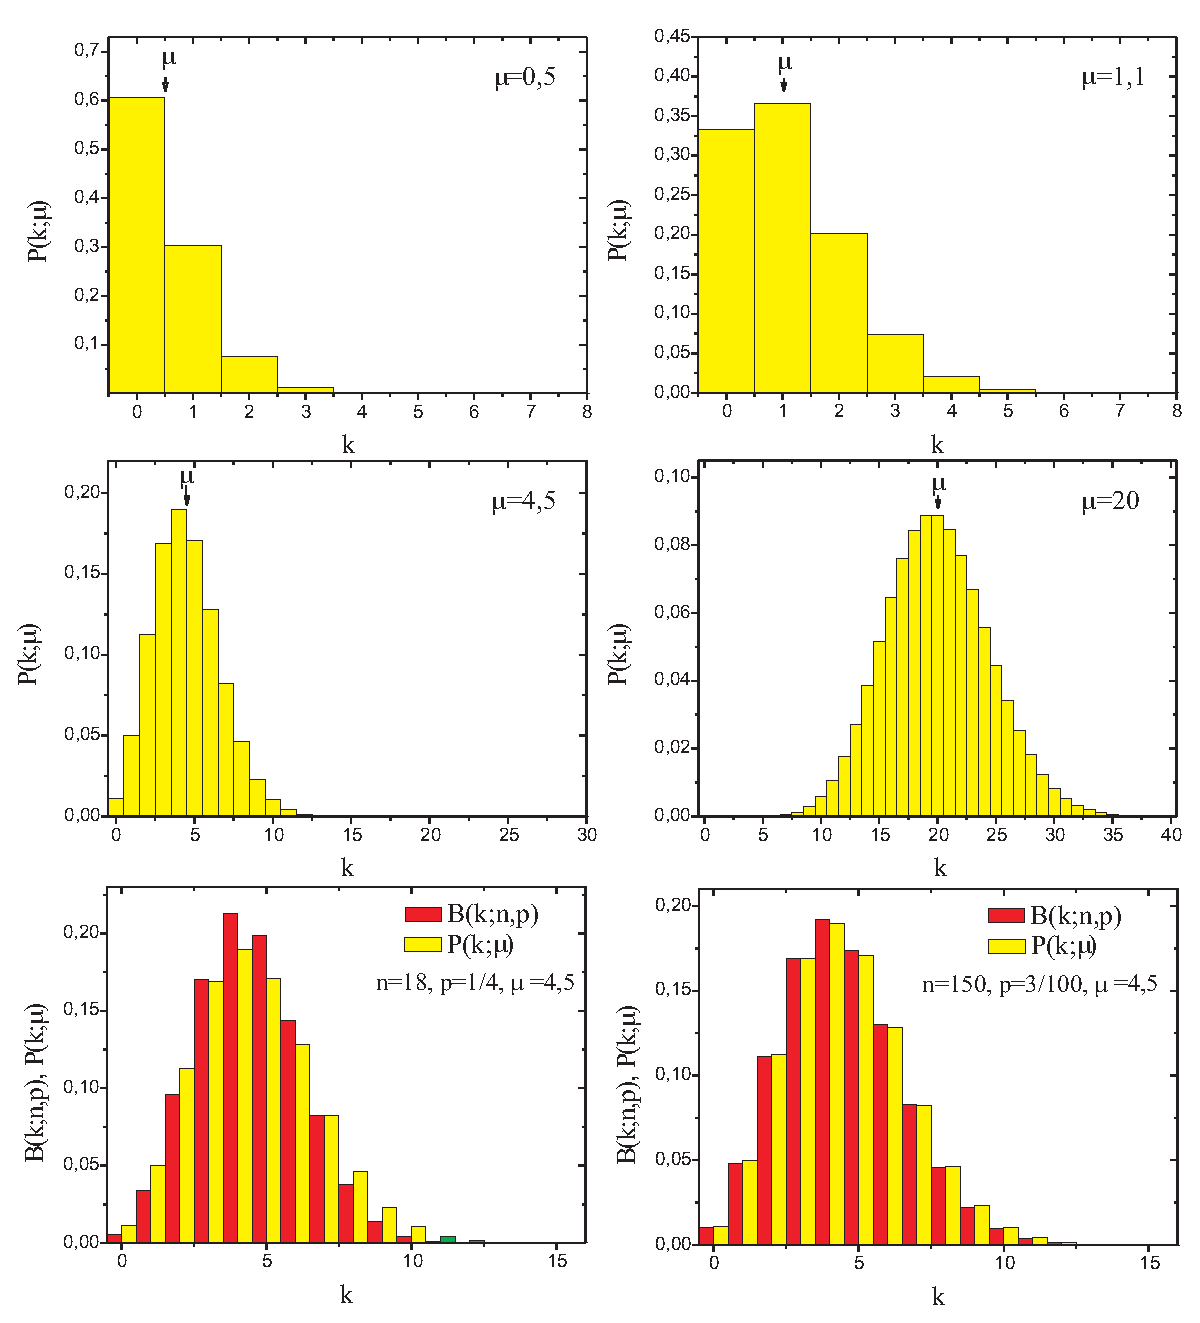
\epsfig{file=251_poisson.eps,width=\textwidth}
\caption{\fontsize{10}{12}\it Poisson-Verteilung f\"{u}r
unterschiedliche Werte von $\mu$. Untere Reihe: Vergleich der
Binomial-Verteilung mit der Poisson-Verteilung. F\"{u}r gro{\ss}e
Werte von $n$ und kleine Wahrscheinlichkeiten $p$ n\"{a}hert sich
die Binomial-Verteilung der
Poisson-Verteilung.\label{251_poisson}}
\end{minipage}
\end{figure}


Die Poisson-Verteilung ist wie die Binomial-Verteilung eine
diskrete Verteilung ($k\in\mathbb{N}$). Sie ist eine
einparametrige Verteilung, die
durch den Mittelwert $\mu$ vollst\"{a}ndig beschrieben wird.\\
\newline
Eigenschaften der Poisson-Verteilung:
\begin{alignat}{2}
&\text{Normierung:}  \quad  &  &\sum_{k=0}^\infty P(k;\mu)=1  \\
&\text{Mittelwert:}  \quad  &\langle k \rangle =&\sum_{k=0}^\infty k\,P(k;\mu) = \mu \\
&\text{Varianz:}    \quad &\sigma^2=&\sum_{k=0}^\infty
k^2\,P(k;\mu)-\langle k \rangle^2= \mu\\
&\text{Standardabweichung:}\quad &\sigma=&\sqrt{\mu}
\end{alignat}
Beachten Sie, dass der Parameter $\mu$ zugleich den Mittelwert als
auch die Varianz darstellt. Die Standardabweichung berechnet sich
demnach aus der Wurzel des Mittelwertes. Hierauf beruht das
$\sqrt{N}$-Gesetz bei der Fehlerbestimmung von gez\"{a}hlten Gr\"{o}{\ss}en.
Wir werden an sp\"{a}terer Stelle noch darauf zur\"{u}ckkommen.


In Abbildung~\ref{251_poisson} ist die Poisson-Verteilung f\"{u}r
verschiedene Werte von $\mu$ dargestellt. F\"{u}r $\mu < 1$ ist der
wahrscheinlichste Wert stets Null. Die Verteilung besitzt in
diesem Fall kein Maximum und nimmt monoton mit zunehmendem $k$ ab.
F\"{u}r $\mu > 1$ besitzt die Verteilung ein Maximum, dessen Breite
allerdings bei gleichem Mittelwert  gr\"{o}{\ss}er ist als die der
Binomial-Verteilung (Die Varianz der Poisson-Verteilung entspricht
dem Mittelwert $\sigma_P^2=\mu\equiv np$, w\"{a}hrend sie bei der
Binomial-Verteilung gegeben ist durch $\sigma_B^2= np\,(1-p) <
\sigma_P^2$). Weiterhin f\"{a}llt auf, dass die Verteilungen f\"{u}r
kleine Mittelwerte stark asymmetrisch sind und f\"{u}r gr\"{o}{\ss}er werdende
Mittelwerte immer symmetrischer werden. In der Tat geht die
Poisson-Verteilung f\"{u}r gro{\ss}e $\mu$ in die symmetrische
Gau{\ss}-Verteilung \"{u}ber.

\subsubsection{Die Gau{\ss}-Verteilung}
F\"{u}r einen gro{\ss}en Mittelwert ($\mu > 30$) l\"{a}sst sich die
Poisson-Verteilung in guter N\"{a}herung durch eine
Gau{\ss}-Verteilung approximieren (Die Herleitung finden Sie
wieder im Anhang):
\begin{equation}\label{251_gauss}
G(k;\mu)=\frac{1}{\sqrt{2\pi\mu}}\,\text{e}^{-\frac{(\mu-k)^2}{2\mu}}.
\end{equation}

Gleichung~(\ref{251_gauss}) stellt ein Spezialfall der
Gau{\ss}-Verteilung dar, bei der die Varianz dem Mittelwert
entspricht. Die allgemeine Form lautet:

\begin{equation}\label{251_gauss2}
   G(k;\mu,\sigma)=\frac{1}{\sqrt{2\pi}\,\sigma}\,\text{e}^{-\frac{(\mu-k)^2}{2\sigma^2}}.
\end{equation}
\newline
Eigenschaften der Gau{\ss}-Verteilung:
\begin{alignat}{2}
&\text{Normierung:}  \quad  &  &\int_{-\infty}^\infty G(k;\mu,\sigma)\,dk=1  \\
&\text{Mittelwert:}  \quad  & &\int_{-\infty}^\infty k\,G(k;\mu,\sigma)\,dk = \mu \\
&\text{Varianz:}    \quad & &\int_{-\infty}^\infty
k^2\,G(k;\mu,\sigma)\,dk -\langle k \rangle^2= \sigma^2
\end{alignat}

F\"{u}r den Spezialfall einer Z\"{a}hlstatistik
(Gleichung~(\ref{251_gauss})) ergibt sich, wie bei der
Poissonverteilung, f\"{u}r die Standardabweichung
\begin{equation}
  \sigma=\sqrt{\mu}.
\end{equation}

\begin{figure}[h]
\begin{minipage}[c]{12cm}
\centering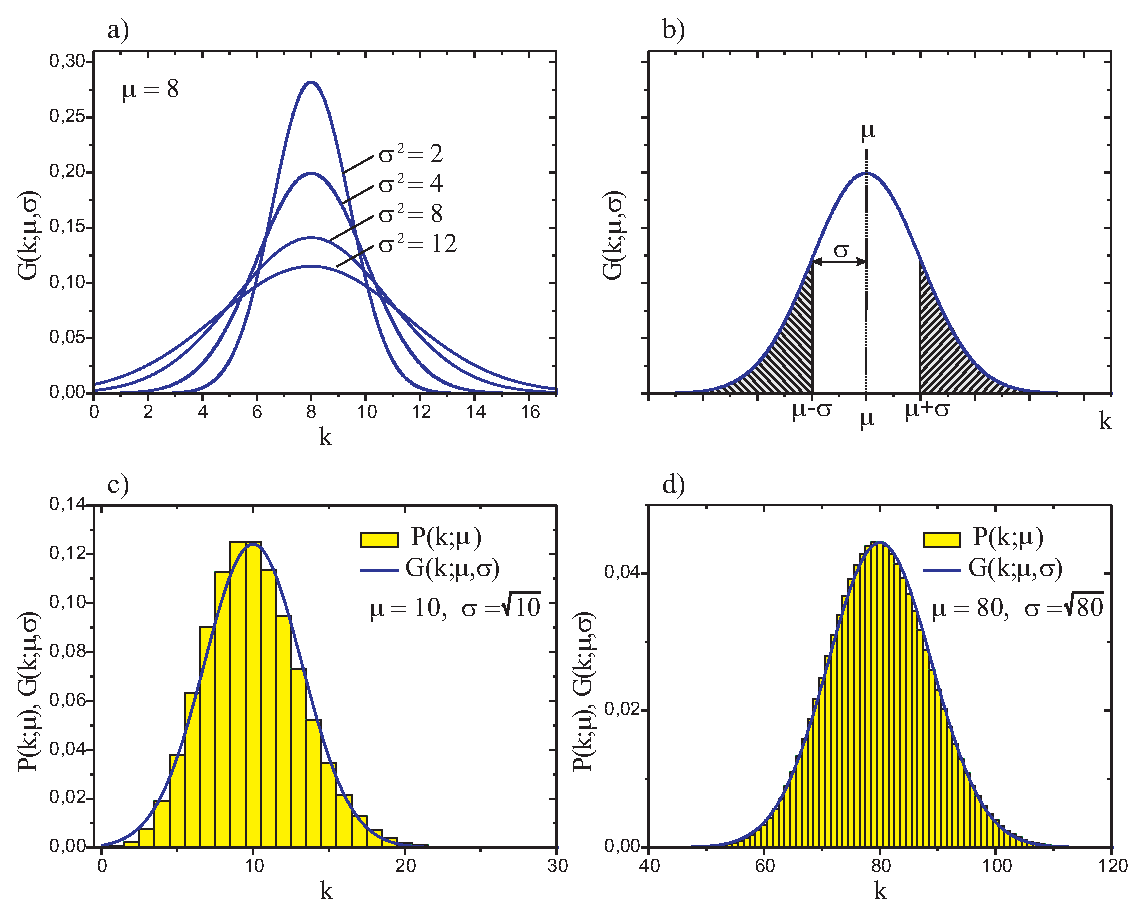
\epsfig{file=251_gauss.eps,width=\textwidth}
\caption{\fontsize{10}{12}\it \label{251_gaussplot} a) Gau{\ss}-
Verteilung f\"{u}r $\mu=8$ und verschiedene Werte von $\sigma$. b)
Grafische Darstellung von $\sigma$. c) und d) Vergleich der
Poisson-Verteilung mit der Gau{\ss}-Verteilung.}
\end{minipage}
\end{figure}


Im Gegensatz zur Binomial- und Poissonverteilung, deren Variable
$k$ nur diskrete Werte annehmen kann, ist die Gau{\ss}-Verteilung
kontinuierlich, d.h. $k\in \mathbb{R}$. Sie ist eine
zweiparametrige Verteilung, die durch den Mittelwert $\mu$ und die
Standardabweichung $\sigma$ eindeutig bestimmt ist. In
Abbildung~\ref{251_gaussplot}a) sind einige Verteilungen mit
unterschiedlichen  Standardabweichungen dargestellt. Je
gr\"{o}{\ss}er die Standardabweichung $\sigma$, desto breiter ist
die Verteilung. Die Bilder c) und d) vergleichen die
Gau{\ss}-Verteilung mit der Poissonverteilung f\"{u}r zwei
unterschiedliche Mittelwerte. In Abbildung~\ref{251_gaussplot}b)
ist eine Gau{\ss}-Verteilung abgebildet, bei der die Fl\"{a}chen
unter der Kurve im Bereich $k>\mu+\sigma$ und $k<\mu-\sigma$
schraffiert dargestellt ist. Diese Fl\"{a}che gibt die
Wahrscheinlichkeit $P_\sigma$ an, dass $k$ um mehr als eine
Standardabweichung vom Mittelwert $\mu$ abweicht. $P_\sigma$
l\"{a}sst sich gem\"{a}{\ss}
\begin{equation}
  P_\sigma= 1-\int_{\mu-\sigma}^{\mu+\sigma} G(k;\mu,\sigma) dk
\end{equation}
berechnen und betr\"{a}gt etwa 30~\%. Analog erh\"{a}lt man die
Wahrscheinlichkeiten f\"{u}r Abweichungen von $\mu$ um mehr als
$\pm 2\sigma$ und $\pm 3\sigma$ (Tabelle~\ref{251_Tab1}).


\begin{table}
\begin{center}
\begin{tabular}{|c|c|c|c|}
\hline
    Eine Abweichung von $\mu$ um mehr als& $\pm \sigma$ & $\pm 2 \sigma$& $\pm 3 \sigma$\\\hline
  hat die Wahrscheinlichkeit &31,73\%&4,55\%&0,27\%\\\hline
\end{tabular}

\caption{\fontsize{10}{12}\it \label{251_Tab1}
Wahrscheinlichkeiten f\"{u}r unterschiedliche Werte von $\sigma$.}
\end{center}
\end{table}



Um auf einfacher Weise die Standardabweichung aus einer
Gau{\ss}kurve abzusch\"{a}tzen, sollten Sie sich folgende
Beziehung merken:
\begin{equation}
FWHM\approx 2,36 \sigma,
\end{equation}
wobei $FWHM$ f\"{u}r \it full width at half maximum\rm~steht, d.h. f\"{u}r
die volle Breite der Kurve auf halber H\"{o}he.

\subsection{Statistik und Messfehler}
In der Praxis ist der Mittelwert $\mu$ einer sehr langen Messreihe
meist nicht gegeben, sondern nur das Resultat $k$ einer einzigen
Messung. In diesem Fall kann man das Ergebnis als Sch\"{a}tzung des
Mittelwertes interpretieren:\\

\textsf{G($\mu$;$k$) ist die Wahrscheinlichkeit, dass eine sehr
lange Messreihe den Mittelwert $\mu$ ergeben w\"{u}rde,
wobei das Resultat $k$ einer einzigen Messung gegeben ist.}\\
\\
Da $k$ und $\mu$ nicht stark voneinander abweichen, k\"{o}nnen wir
aufgrund einer einzigen Messung auch einen N\"{a}herungswert f\"{u}r die
Standardabweichung angeben:
\begin{equation}
   \sigma = \sqrt{k}.
\end{equation}
Es ist \"{u}blich, das Resultat einer solchen Z\"{a}hlung in der Form
\begin{equation}
  k \pm\sqrt{k}
\end{equation}
anzugeben. Dies ist eine Abk\"{u}rzung f\"{u}r die S\"{a}tze: \glqq Ich habe
$k$ Ereignisse gez\"{a}hlt. Daraus schlie{\ss}e ich, wegen
Abbildung~\ref{251_gaussplot}b) und Tabelle~\ref{251_Tab1}, dass
der Mittelwert einer sehr langen Messung mit 68\%
Wahrscheinlichkeit im Bereich $k \pm\sqrt{k}$ liegt, mit 95\%
Wahrscheinlichkeit im Bereich $k \pm 2\sqrt{k}$ und nur mit einer
Wahrscheinlichkeit von 0,3\% au{\ss}erhalb des Bereichs $k \pm
3\sqrt{k}$\grqq.

Die Betrachtung der statistischen Fehler ist besonders wichtig,
wenn man he\-rausfinden will, ob die Differenz zweier
Z\"{a}hlergebnisse $k_1$ und $k_2$, allein durch statistische
Schwankungen erkl\"{a}rt werden kann oder auf eine \"{A}nderung der
Versuchsbedingungen zur\"{u}ckzuf\"{u}hren ist. Viele Experimente laufen
auf diese Fragestellung hinaus.

Nach dem Fehlerfortpflanzungsgesetz erh\"{a}lt man den mittleren
statistischen Fehler einer Differenz durch quadratisches Addieren
der Einzelfehler.

Es sei
\begin{equation}
  \Delta = k_1 - k_2;\quad \sigma_1 = \sqrt{k_1};\quad \sigma_2 = \sqrt{k_2}.\notag
\end{equation}
Dann ist
\begin{equation}
  \sigma_\Delta = \sqrt{\sigma_1^2 + \sigma_2^2} = \sqrt{k_1 + k_2}.\notag
\end{equation}

Man schreibt dies meist in der Form :

\begin{equation}
\Delta = (k_1 - k_2) \pm \sqrt{k_1 + k_2}.\notag
\end{equation}

F\"{u}r die Wahrscheinlichkeit, dass $\Delta$ allein aufgrund von
statistischen Schwankungen  von Null um mehr als eine, zwei oder
drei Standardabweichungen ($\sigma_\Delta = \sqrt{k_1 + k_2}$)
abweicht, gilt wieder Tabelle~\ref{251_Tab1}. In der Regel h\"{a}lt
man den Einfluss einer \"{A}nderung der Versuchsbedingungen f\"{u}r
erwiesen, wenn $\Delta$ um mehr als drei Standardabweichungen von
Null abweicht. In diesem Fall bezeichnet man die Differenz
$\Delta$ als \bf signifikant\rm.



\section{Durchf\"{u}hrung des Versuchs}
\begin{enumerate}

\item Skizzieren Sie den Versuchsaufbau.

\item \it Messung der Z\"{a}hlrohrcharakteristik\rm \\
\\
Messen Sie die Z\"{a}hlrohrcharakteristik mit Hilfe des internen
Z\"{a}hlers des Betriebsger\"{a}tes. Das Pr\"{a}parat ($^{60}$Co oder
$^{137}$Cs) erhalten Sie vom Versuchsbetreuer. Folgen Sie dazu den
Anweisungen in den Abschnitten \glqq Inbetriebnahme des
Z\"{a}hlger\"{a}tes - Einstellung der Einsatzspannung\grqq~und \glqq
Messung des Z\"{a}hlrohrplateaus\grqq~in der Beschreibung \it
Grundlagen zu den Versuchen der Radioaktivit\"{a}t\rm. Tragen Sie die
Messwerte  mit den statistischen Fehlern sofort in ein Diagramm
ein. Stellen Sie nach der Messung die Z\"{a}hlrohrspannung auf die
Mitte des gemessenen Plateaubereichs ein. Dieser Spannungswert
wird im Folgenden als $U_0$ bezeichnet.

\item  \it Untersuchung des Plateauanstiegs\rm \\
\\Bringen Sie das Pr\"{a}parat m\"{o}glichst dicht an das Z\"{a}hlrohr und
messen Sie jeweils 1~Minute und 3~Minuten lang die Z\"{a}hlrate bei
den Spannungen $U_0$ und $U_0 + 100$~V. Stellen Sie
anschlie{\ss}end die Z\"{a}hlrohrspannung wieder auf $U_0$ ein.

\item \it Verifizierung der statistischen Natur des radioaktiven Zerfalls\rm \\

In dieser Teilaufgabe werden Sie viele Male (mindestens 2000~Mal)
die Zerf\"{a}lle eines radioaktiven Pr\"{a}parats innerhalb eines festen
Zeitraums (Torzeit) messen und in ein Histogramm darstellen. Falls
sich der radioaktive Zerfall v\"{o}llig statistisch verh\"{a}lt, sollte
das gemessene Histogramm durch eine Poisson- Verteilung, bzw. bei
einem gro{\ss}en Mittelwert, durch eine Gau{\ss}- Verteilung beschrieben
werden k\"{o}nnen. \"{U}berpr\"{u}fen Sie dies zun\"{a}chst f\"{u}r einen gro{\ss}en
Mittelwert:

N\"{a}hern Sie das Pr\"{a}parat durch Verschieben des Reiters dem Z\"{a}hlrohr
an, bis etwa 140-150~Zerf\"{a}lle/Sekunde gez\"{a}hlt werden. Die Z\"{a}hlrate
darf auf keinen Fall gr\"{o}{\ss}er gew\"{a}hlt werden, da sonst die Totzeit
des Z\"{a}hlrohres die Statistik verf\"{a}lscht!  Schalten Sie den
Computer und das externe Z\"{a}hlger\"{a}t ein und starten Sie das
Messprogramm \it Statistik.vi\rm~auf dem Desktop. Stellen Sie die Messzeit (Torzeit) auf
500~ms. Starten Sie die Messung durch Dr\"{u}cken des Pfeilsymbols in
der linken oberen Ecke. Die registrierten Zerf\"{a}lle/Torzeit werden
in einem Histogramm dargestellt. Zus\"{a}tzlich wird aus den Messdaten
der Mittelwert und die Standardabweichung berechnet und im Feld
\glqq Statistik\grqq~angezeigt. Der theoretisch zu erwartende Wert
der Standardabweichung ($\sigma_{theor}$) wird aus der
Quadratwurzel des Mittelwertes berechnet und ebenfalls angezeigt.
Wenn Sie die Option \glqq Gau{\ss}kurve\grqq~im Feld \glqq
Einstellungen\grqq~einschalten, wird aus dem gemessenen Mittelwert
und der Standardabweichung die dazugeh\"{o}rige Gau{\ss}-Verteilung
berechnet und im Histogramm mitangezeigt. Beachten Sie, dass die
angezeigte Gau{\ss}kurve nicht angefittet wird, sondern aus den
Messdaten berechnet wird! Die Darstellung der Poisson- Verteilung
ist nur dann m\"{o}glich, wenn der Stoppwert der Abszisse kleiner als
34 ist.

Den Abszissenbereich des Histogramms k\"{o}nnen Sie durch den
Start- und Stoppwert in der linken und rechten unteren Ecke
einstellen. Warten Sie zun\"{a}chst etwa 50~Messungen ab und
stellen Sie dann diese Werte so ein, dass das Histogramm optimal
dargestellt wird.

\bf Insgesamt sind  mindestens 2000~Messungen
durchzu\-f\"{u}h\-ren.\rm~W\"{a}hrend dieser Zeit k\"{o}nnen Sie mit der
Auswertung der Aufgaben~2 und~3 beginnen.  Zum Beenden der Messung
dr\"{u}cken Sie die Stop-Taste im Feld \glqq Aktuelle Messung\grqq.
Notieren Sie die gemessenen Werte (Anzahl der Messungen,
Mittelwert und Standardabweichungen) und f\"{u}hren Sie sofort die
Auswertung (Teil 4a im Kapitel Auswertung) durch.


\item \it Vergleich der Poisson- und Gau{\ss}- Verteilung bei sehr kleinen Z\"{a}hlraten\rm \\
\\Stellen Sie das abgeschirmte Pr\"{a}parat so in die N\"{a}he des
Z\"{a}hlrohrs, dass etwa 40 - 50 Teilchen/Sekunde gez\"{a}hlt werden.
Stellen Sie die \bf Messzeit auf 100~ms\rm~ein und starten Sie die
Messung. \bf Insgesamt sind mindestens 5000~Messungen
durchzu\-f\"{u}h\-ren.\rm~Notieren Sie nach Beendigung der Messung die
gemessenen Werte (Anzahl der Messungen, Mittelwert und
Standardabweichungen) und f\"{u}hren Sie sofort wieder die Auswertung
durch.


\end{enumerate}

\section{Auswertung}

\begin{usingpython}
Führen Sie die Rechnungen in einem vollständig dokumentierten Jupyter Notebook durch und legen Sie es Ihrem Laborbuch anschließend ausgedruckt bei.
\end{usingpython}

\begin{usingorigin}
Da es im Laborbuch nicht m\"{o}glich ist nachzuvollziehen, welche Rechnungen Sie mit Origin durchgef\"{u}hrt haben, muss bei allen Spaltenberechnungen die entsprechende Rechenvorschrift (Formel) im Laborbuch kommentiert werden.
\end{usingorigin}

\begin{itemize}
  \item Plateaubereich des Z\"{a}hlrohrs.\\
  \\Werten Sie die Differenzen $(n(U_0+100~V) - n(U_0))$  bei den jeweiligen Messzeiten aus und
  berechnen Sie f\"{u}r beide Zeitintervalle den prozentualen Anstieg der Z\"{a}hlrate pro 100~V mit dem dazugeh\"{o}rigen
  statistischen Fehler:
  \begin{itemize}
    \item [a)]	Ist der gemessenen Anstieg signifikant?
    \item [b)]	Welche prozentuale Variation der Z\"{a}hlrate ist bei einer Spannungserh\"{o}hung um 100 V m\"{o}glich bei einem Vertrauensniveau von ca. 68$\%$ und von ca. 95$\%$?
    \item [c)]	Wie lange m\"{u}ssten Sie messen um den Plateauanstieg auf 1 $\%$ genau zu kennen?
  \end{itemize}
  \item  Auswertung der Daten mit hoher mittlerer Ereigniszahl.

  Die Daten der Messreihe wurden vom Messprogramm in die Datei  \verb"Statistik.dat" im Ordner  \verb"Messungen"  auf dem Desktop gespeichert. Der Datensatz besteht aus zwei Spalten, der Anzahl der Zerf\"{a}lle/Zeiteinheit und deren H\"{a}ufigkeit.
  
  \begin{usingorigin}
    Starten Sie das Programm \verb"Origin" vom Desktop aus und importieren Sie die Messdaten:
\verb"Datei" $\rightarrow$ \verb"Importieren" $\rightarrow$ \verb"Einzelnes ASCII". Beschriften Sie die Spalten und erzeugen Sie eine weitere Spalte (\verb"Spalte" $\rightarrow$ \verb"Spalten hinzufuegen") mit den statistischen Fehlern. Der statistische Fehler berechnet sich aus der Quadratwurzel der gemessenen Ereignisse: Dazu die zu berechnende Spalte markieren, Rechtsklick auf den Spaltenkopf $\rightarrow$ \verb"Spaltenwerte errechnen" ausw\"{a}hlen und die entsprechende Formel angeben. Setzen Sie diese Spalte als  Y-Fehlerbalken: \verb"Spalte" $\rightarrow$ \verb"Setzen als" $\rightarrow$ \verb"Y-Fehler" und beschriften Sie diese entsprechend.

Zeichnen Sie von den Daten ein Punktdiagramm mit Fehlerbalken (alle Spalten ausw\"{a}hlen  $\rightarrow$ \verb"Zeichnen" $\rightarrow$ \verb"Symbol" $\rightarrow$ \verb"Punktdiagramm"). Stellen Sie geeignete $x$- und $y$-Bereiche ein.
\end{usingorigin}

Fitten Sie an die Daten eine Gaussfunktion gem\"{a}{\ss}:

\begin{equation}\notag
    y= A/\text{sqrt}(sig^\wedge 2*2*3.14)*\text{exp}(-(x-xc)^\wedge 2/2/sig^\wedge2),
\end{equation}

mit den freien Parametern $sig, xc$ und $A$. Diese Funktion ist nicht als \verb"OriginBasicFunction" verf\"{u}gbar sondern muss sp\"{a}ter von Ihnen als neue Funktion programmiert werden.


Datenauswahl: der genutzte $\chi^2$-Fit funktioniert nur, wenn die Fehler \glqq gaussverteilt\grqq~sind. Das ist in hinreichendem Ma{\ss}e nur dann der Fall, wenn die H\"{a}ufigkeit mindestens zehn betr\"{a}gt. Dies werden Sie u.a. in diesem Versuch lernen. Nutzen Sie daher das Datenauswahlwerkzeug: Klicken Sie auf  \begin{minipage}{5mm}
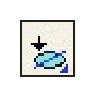
\includegraphics[height=5mm]{icon_auswahl.eps}\end{minipage} und ziehen Sie im Diagramm ein Rechteck um die Daten. Es erscheinen zwei Pfeilmarken. Darauf klicken und mit dem Haarkreuz \"{u}ber die Daten schieben. X und Y-Werte werden in einem kleinen Fenster angezeigt. Verschieben Sie beide Pfeile so lange, bis Sie einen Y-Wert (H\"{a}ufigkeit) von mindestens 10 erreicht haben.



Fitprozedur: Starten Sie die Fitroutine mit \verb"Analyse"  $\rightarrow$ \verb"Anpassen" $\rightarrow$ \verb"Nichtlinearer Fit" $\rightarrow$ \verb"Dialog oeffnen". F\"{u}hren Sie im Dialogfenster folgende Schritte durch:
\begin{enumerate}
  \item Auf \verb"Funktionsauswahl" klicken und im Feld \verb"Funktion" den Eintrag \verb"<Neu...>" ausw\"{a}hlen.
  \item Geben Sie im Feld \verb"Funktionsname" einen sinnvollen Namen ein. Entsprechend m\"{u}ssen Sie im Feld \verb"Parameter" die Fitparameter (mit Komma getrennt) eintragen und im Feld \verb"Funktion" die Fitfunktion eintippen. Danach auf \verb"Speichern" und \verb"OK"  klicken.
  \item  Im Dialogfenster \verb"NLFit"  auf \verb"Datenauswahl" klicken: Nacheinander auf die Optionen
\verb"Bereich 1", \verb"y" und \verb"Gewichtung" klicken. Unter Zeilen sollten die von Ihnen ausgew\"{a}hlten Start- und Stoppzeilennummer stehen.  Notieren Sie sich diese Werte als \glqq Fitbereich\grqq.

\item Klicken Sie auf das Registerblatt \verb"Parameter" und tragen Sie unter \verb"Wert" Ihre Sch\"{a}tzwerte der Fitparameter ein:  \verb"A"=Gesamtzahl der Ereignisse, \verb"xc" = Mittelwert (Maximum) und \verb"sig =" $\sqrt{xc}$. Sie k\"{o}nnen auch f\"{u}r \verb"A" die gesamte Zahl der registrierten Zerf\"{a}lle einsetzen und den Parameter fixieren. Klicken Sie danach auf den Knopf \begin{minipage}{5mm}
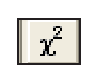
\includegraphics[height=4mm]{icon_chi2.eps}\end{minipage} und beobachten Sie wie eine Kurve in Ihr Diagramm gezeichnet wurde. Falls Sie keine Kurve sehen, m\"{u}ssen Sie die Parameter entsprechend \"{a}ndern.  Klicken Sie nun mehrfach auf den daneben liegenden Knopf \begin{minipage}{5mm}
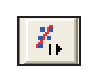
\includegraphics[height=4mm]{icon_1it.eps}\end{minipage} f\"{u}r eine Iteration und beobachten Sie gleichzeitig die Fitkurve im Diagramm und den Wert von $\chi^2$ im Nachrichtenfenster. Falls der Fit nicht konvergiert, m\"{u}ssen Sie bessere Parameter w\"{a}hlen.
  \item Gehen Sie zur\"{u}ck zum Registerblatt \verb"Einstellungen" und w\"{a}hlen Sie den Eintrag \verb"Fit-Kurven"  aus.
Ohne weitere Auswahl wird die Fitkurve nur innerhalb des ausgew\"{a}hlten Datenbereichs gezeichnet. Hier ist es allerdings sinnvoll die Fitkurve \"{u}ber den gesamten Datenbereich zu zeichnen. W\"{a}hlen Sie unter \verb"Angepasstes Kurvendiagramm" $\rightarrow$ \verb"X-Datentyp" $\rightarrow$ \verb"Bereich" die Option
\verb"Ausweiten auf gesamten Achsenbereich" aus. Klicken Sie nun auf den Knopf \verb"Fit". Schauen Sie sich die detaillierten Fitresultate an und notieren Sie sich die Parameter, deren Fehler und alle sonst wichtigen Ergebnisse ($\chi^2$) in Ihr Laborbuch.

\item Drucken Sie das Diagramm aus und f\"{u}gen Sie es in Ihr Laborbuch ein.
\end{enumerate}

\item Anpassung einer Poissonverteilung an die Daten.\\
\\Wiederholen Sie die Fitprozedur f\"{u}r dasselbe Diagramm indem Sie jetzt eine
Poissonverteilung anpassen. Hierzu m\"{u}ssen Sie wieder eine neue Fitfunktion definieren:
\begin{equation}\notag
   y= A* exp(-mu)* mu^\wedge x / gamma(x+1).
\end{equation}
Dabei k\"{o}nnen Sie den Parameter A auf die Gesamtzahl aller Zerf\"{a}lle normieren und
nur den Parameter \verb"mu" fitten.  \verb"mu" ist die mittlere erwartete Ereigniszahl im
Zeitintervall. Hinweis: die Gammafunktion hat den Funktionswert $n!$ f\"{u}r alle nat\"{u}rlichen
Zahlen, ist aber f\"{u}r alle reellen Zahlen definiert.

Sie sollten jetzt zwei Fitkurven im Diagramm
sehen. \"{A}ndern Sie den Linientyp (z.B. punktiert) der Poissonfunktion im Diagramm.
Die Unterschiede der beiden Fitfunktionen sind besonders gut sichtbar, wenn Sie in eine
logarithmischen Darstellung w\"{a}hlen. Doppelklick auf die y-Achse und bei \verb"Art" \verb"Log10" ausw\"{a}hlen. Drucken Sie das
Diagramm aus und heften Sie es in Ihr Laborbuch.

\item
Auswertung der Messdaten mit kleiner mittlerer Ereigniszahl.\\
\\Wiederholen Sie alle zuvor durchgef\"{u}hrten Schritte f\"{u}r den neuen Datensatz mit kleiner mittlerer Ereigniszahl.
\"{O}ffnen Sie hierzu eine neue Arbeitsmappe.  Speichern Sie am Ende das ganze Projekt mit eigenem
Dateinamen.

\item Diskussion der Ergebnisse.\\
\\
Diskutieren Sie das Ergebnis der beiden Messungen und deren Auswertung!
Wie gut sind die Wahrscheinlichkeiten der gefitteten Verteilungen. Diskutieren Sie insbesondere das jeweilige reduzierte $\chi^2$. Wann kann eine Messreihe, die statistisch verteilte Ereignisdaten liefert, mit einer Gaussverteilung angen\"{a}hert werden? Welche Werte haben dann der Mittelwert $\mu$ und die Breite $\sigma$?
Wo liegen  die systematischen Unterschiede zwischen Gauss- und Poissonverteilung. Warum sind die statistischen Fehler f\"{u}r kleine Erwartungswerte nicht gaussverteilt?

\end{itemize}


\section{Anhang}
\subsection{Die Poisson-Verteilung als Grenzfall der Binomial-Verteilung}
Bezeichnen wir den Mittelwert von $k$ mit $\mu \equiv np$, so
l\"{a}sst sich die Binomial-Verteilung
\begin{eqnarray}
B(k;n,p)&=&\binom{n}{k}p^k (1-p)^{n-k}\\
&=&\frac{n!}{k!\,(n-k)!}\, p^k (1-p)^{n-k}
\end{eqnarray}
wie folgt umformen. Mit p=$\mu$/n ergibt sich
\begin{eqnarray}
B(k;n,p)&=&\frac{n!}{k!\,(n-k)!}\, \frac{\mu^k}{n^k}
\biggl(1-\frac{\mu}{n}\biggr)^{n-k}\\
&=&\biggl\{\frac{n!}{(n-k)!}\,\frac{1}{n^k}\biggr\}\,\biggl(1-\frac{\mu}{n}\biggr)^{-k}\frac{\mu^k}{k!}
\biggl(1-\frac{\mu}{n}\biggr)^{n}\label{251_P4}.
\end{eqnarray}
F\"{u}hren wir nun den Grenz\"{u}bergang $n\rightarrow\infty$ und
$p\rightarrow 0$ durch, mit der Forderung das $\mu=np$ endlich
bleibt, so konvergieren die ersten beiden Faktoren gegen Eins. F\"{u}r
den zweiten Faktor ist dies sofort einzusehen. F\"{u}r den ersten
Ausdruck in der geschweiften Klammer gilt f\"{u}r $n\gg k$:
\begin{equation}
\frac{n!}{(n-k)!}= n\cdot(n-1)\cdot(n-2)\cdot ... \cdot
(n-k+1)\approx n^k
\end{equation}
und somit
\begin{equation}
\lim_{n\rightarrow\infty}\biggl\{
\frac{n!}{(n-k)!}\,\frac{1}{n^k}\biggr\}=1.
\end{equation}

Der letzte Faktor in Gleichung~(\ref{251_P4}) konvergiert
 gegen die Exponentialfunktion mit dem Argument $-\mu$.
Somit erhalten wir schlie{\ss}lich die Poisson-Verteilung:


\begin{equation}
P(k;\mu)=\frac{\mu^k}{k!}\,\text{e}^{-\mu}.
\end{equation}

\subsection{Die Gau{\ss}- Verteilung als Grenzfall der Poisson- Verteilung}

F\"{u}r gro{\ss}e Mittelwerte ($\mu > 30$) geht die Poisson- Verteilung in
eine Gau{\ss}- Verteilung \"{u}ber. Ersetzen wir die Fakult\"{a}t in der
Poisson- Verteilung durch die Stirling'sche N\"{a}herungsformel
\begin{equation}
k! = \sqrt{2\pi k}\, k^k \,\text{e}^{-k},
\end{equation}
so ergibt sich

\begin{eqnarray}
P(k;\mu)&=&\frac{\mu^k}{k!}\,\text{e}^{-\mu} \rightarrow \frac{\mu^k \,\text{e}^{-\mu}}{\sqrt{2\pi k}\, k^k\, \text{e}^{-k}} = \frac{\text{e}^{-(\mu-k)}}{\sqrt{2\pi \mu}}\biggl(\frac{\mu}{k} \biggr)^{k+\frac{1}{2}}\\
&=& \frac{\text{e}^{-(\mu-k)}}{\sqrt{2\pi \mu}}\biggl(1+\frac{\mu
- k}{k}\biggr)^{k+\frac{1}{2}}\\
&=& \frac{\text{e}^{-(\mu-k)}}{\sqrt{2\pi \mu}}\,
\exp\biggl\{\biggl(k + \frac{1}{2}\biggr)\, \ln\biggl(1 +
\frac{\mu - k}{k}\biggr)\biggr\}
\end{eqnarray}


Entwickeln wir den Logarithmus nach Taylor
\begin{equation}
\ln(1 + x) = x - \frac{x^2}{2} + \frac{x^3}{3} - \frac{x^4}{4} +
...
\end{equation}

und brechen nach dem quadratischen Glied ab, so erhalten wir
\begin{equation}
P(k;\mu) \rightarrow \frac{\text{e}^{-(\mu-k)}}{\sqrt{2\pi \mu}}\,
\exp\biggl\{\biggl(k+\frac{1}{2}\biggr)\biggl(\frac{\mu - k}{k}\,-
\frac{1}{2}\frac{(\mu -k)^2}{k^2}\biggr)\biggr\}.
\end{equation}
Bei hinreichend gro{\ss}em $k$ k\"{o}nnen wir $k+1/2$ durch $k$ ersetzen
und erhalten damit
\begin{equation}
P(k;\mu) \rightarrow \frac{1}{\sqrt{2\pi
\mu}}\,\text{e}^{-\frac{(\mu-k)^2}{2k}}.
\end{equation}
Da $(\mu-k)/k \ll 1$ k\"{o}nnen wir im Nenner des Exponenten $k$ durch
$\mu$ ersetzen und erhalten schlie{\ss}lich einen Spezialfall der
Gau{\ss}- Verteilung mit $\sigma=\sqrt{\mu}$ :
\begin{equation}
G(k;\mu) = \frac{1}{\sqrt{2\pi
\mu}}\,\text{e}^{-\frac{(\mu-k)^2}{2\mu}}.
\end{equation}

\newpage$\quad$
\begin{figure}
\begin{minipage}[c]{22cm}
\centering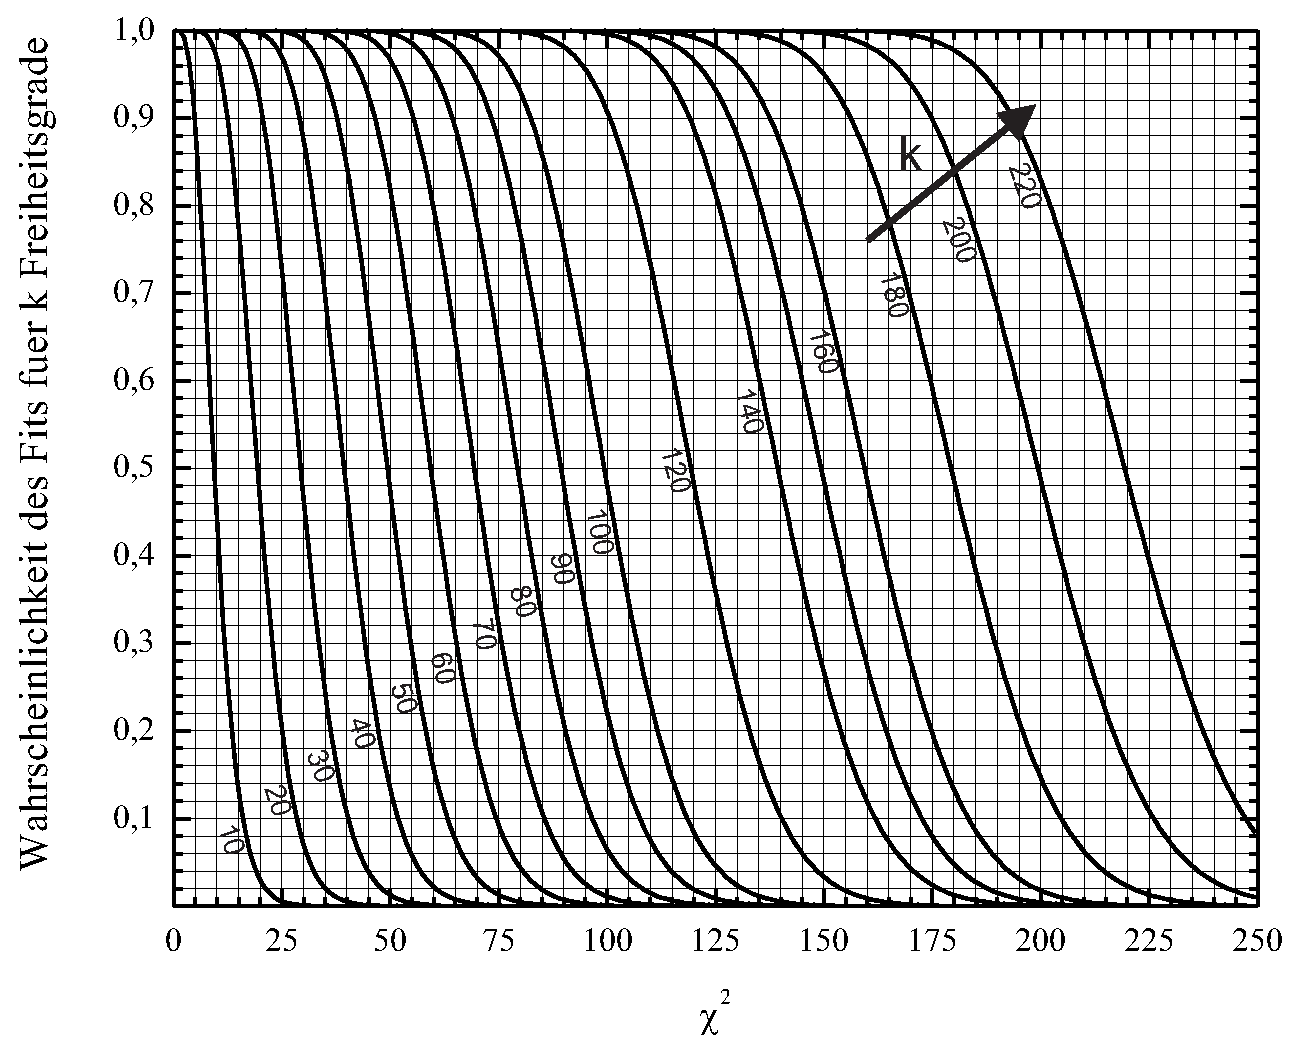
\epsfig{file=251_chi2.eps,width=18cm}
\centering\caption{\fontsize{10}{12}\it
Fitwahrscheinlichkeiten. Der Parameter $k$ gibt die Anzahl der Freiheitsgrade an.}
\end{minipage}
\end{figure}

 \setcounter{section}{0}

\setcounter{figure}{0}

\setcounter{equation}{0}

\setcounter{footnote}{0}

 \setcounter{section}{0}
\end{document}
http://www.strz.uni-giessen.de/ExpHelp/wqa/wqa.html#Totzeitkorrektur_002dRechnungen
http://medweb.uni-muenster.de/institute/imib/lehre/skripte/biomathe/bio/script5.html
http://www.physik.unizh.ch/~lehnerf/lecture/statistik/script.pdf
